This chapter motivates and defines \emph{Persistent Memory Consistency}.
This should be considered future work and I welcome feedback.
I first define the problem and then give examples of persistent memory consistency models.
In the next chapter I give examples of programming patterns, why they require relaxed persistent consistency models, and possible optimizations.

\section{Introduction}
\label{sec:PMC:Intro}

Future NVRAMs will provide a persistent store with the programming interface of modern main memories.
While such technologies could revolutionize the design of recoverable systems and durable storage, questions remain regarding device performance and the NVRAM programming model.
Chapters~\ref{chap:OLTP_design} and~\ref{chap:OLTP_eval} considered an abstract \emph{persist barrier} capable of enforcing persist order or blocking until previous persists complete.
Instead of considering an implementation or exact semantics of these barriers, I instead looked at the effect average persist barrier latency had on OLTP software design.
This project delves into the details of persist barriers, considering their implementation, performance impact, and programming model.

Persist barriers exist as a tool for programmers to ensure correct persistence behavior, while at the same time improving performance.
Without persist barriers, all persists must truly occur in program order for the programmer to reason about persistent state.
This is in fact a popular model for DRAM programming, but the volatile semantics of DRAM allows writes to execute to fast, volatile caches.
NVRAM persists, on the other hand, must always execute to a long latency memory; executing all NVRAM persists in-order introduces frequent, substantial stalls.
Persist barriers remove these stalls by allowing all persists between barriers to occur in parallel.
This is a prime example of using a more complicated programming model to provide performance optimizations.

An altnernative mechanism to enforce persist order is to flush select cache lines or flush the entire cache, either blocking until all data persists or receiving an acknowledgement/interrupt.
This model most closely matches existing disk interfaces -- The programmer invokes system calls to write individual pages and then calls a sync system call.
However, this is a poor match for memory, where the programmer often has little control over how data is laid out (nor do we want programmers to reason about memory/cache architecture).
Instead, we would like a more natural approach to reasoning about persistence that fits existing memory-programming models.

Additional questions remain when memory is shared between threads or processes.
Currently, memory consistency models define how threads communicate and what barriers are necessary to ensure expected behavior.
Memory consistency models exist because processors (and compilers) prefer to run instructions out of order -- a pervasive optimization that significantly complicates multi-threaded programming.
While consistency models control the order in which threads observe reads and writes, there is no similar definition for the order in which persists occur, or how persist order is determined across communicating threads.
Furthermore, persistent memories often care about the actual timing of persists, not just relative ordering -- for example, system calls must make sure that all previous persists have completed before communicating to the outside world.
In this case there is no alternative but to block until all data persists.
These mechanisms are not present in existing consistency models.

While memory consistency models provide a starting point for considering persistent consistency models, the performance differences of volatile memory systems/DRAM and NVRAM will require new programming models for NVRAM.
In fact, the consistency and persistence models may be de-coupled.
That is, the rules that define load and store order might be differ between how \emph{values} are communicated and how \emph{persist order} is enforced.

I wish to extend memory consistency models with persistence semantics to address these concerns.
My goals are to determine how multi-threaded consistency interacts with persistence, how to relax persistent consistency models to provide high performance and an easily programmable interfaces, and identify programming patterns likely to cause NVRAM performance bottlenecks alongside potential optimizations.
All of these will eventually lead to the design of new persistent memory consistency models and implementations, yet that is outside the scope of this project.

The remainder of this chapter describes performance concerns for NVRAM and provides a brief background of memory consistency models before considering simple examples of persistent memory consistency models.
In addition, I examine previous work, highlighting strengths and weaknesses, and placing it into my persistent memory consistency taxonomy.

\section{Performance}
\label{sec:PMC:Performance}

Here I describe how I expect NVRAM, the memory system, and the programming model to affect performance.
Later sections will use these assumptions to reason about consistency model and data structure performance.

There are primarily two cases where persists may cause a thread to stall: ordering barriers and sync barriers.
Ordering barriers may operate by stalling at the barrier until all previous persists complete, obviously stalling the thread of execution.
More complex memory systems will allow threads to continue executing ahead of persistent state, using a buffer to store persists (either in the cache or a memory buffer).
While decoupling volatile execution state and persistent state removes immediate stalls, these buffers may fill, forcing threads to stall until room becomes available.
Therefore, persist throughput is the primary concern -- buffers allow threads to execute ahead of persistent state, but the average rate of persist must match the average rate of execution, otherwise stalls necessarily occur.

Persist throughput is primarily limited by the number of persist dependencies in an applications.
NVARM memories will likely allow high throughput so long as persists may occur in parallel.
Persist dependencies reduce parallelism, requiring that some set of writes persist entirely before any dependent persists begin (necessary for proper recovery).
Since NVRAM cells may take up to microseconds to persists the longest dependence chain of persists will limit persist throughput, additionally limiting execution throughput when buffers fill.
Persistent memory consistency models stand to improve throughput and reduce stalls by relaxing persist ordering constraints, minimizing the persist critical path to only the persist order dependencies necessary.
The ultimate goal is to reduce persist critical path sufficiently that persist throughput exceeds execution throughput, providing the throughput of a DRAM system with the persistence of NVRAM.

Persistent memory applications also introduce stalls at sync barriers.
These are barriers used when interacting with the outside world (e.g., displaying something on-screen, communicating over the network).
Unless this external communication can be asynchronously ordered with persists, allowing the thread to continue doing other useful work, the thread must stall for previous persists to complete, reducing throughput.
Additionally, end-to-end latency is important for many applications and tasks -- greater sync time (while persists drain/flush) leads to increased task latency.
Again, persist critical path determines sync latency; if all independent writes persist in parallel the time to sync is determined by the longest chain of persists outstanding at the time sync is called.

Finally, a persistent memory consistency model may reduce performance if barriers intended to enforce persists order additionally enforce constraints on volatile execution (e.g., a persist barriers prevents memory instructions to volatile addresses from reordering).
While I do not discuss this phenomenon further, I would like to investigate its effects in the future and would appreciate feedback.

This chapter will propose persistent memory consistency models to relax persist constraints and improve NVRAM performance.
First, however, I give a background in existing memory consistency models.
This motivates why persistent consistency models will be important, what sort of consistency relaxations might improve performance, and what sorts of mechanisms ensure correctness when consistency is relaxed.
Additionally, whereas persistent memory consistency models determine persist order, we still require volatile memory consistency models to determine execution \emph{values} and to propagate persist order dependencies between threads.

\section{Memory consistency models}
\label{sec:PMC:MemoryConsistency}

This section provides a background on memory consistency models, focusing on two simple models: Sequential Consistency (SC) and Total Store Order (TSO).
For the remainder of this section I am referring solely to volatile writes without considering for NVRAM persists.
This discussion assumes that caches are completely coherent -- that is, any two accesses to a cache line (by any core/thread), where at least one access is a store, have a total order.
While some relaxed memory models may allow reading of stale cached values, I do not consider that here.

Consistency models define the order that threads observe loads and stores.
While every thread observes its own execution in program order, it may appear that remote threads execute out of order.
Processors (and compilers) are free to reorder instructions to accelerate performance so long as they produce equivalent results.
When examining a program ordering restrictions can be observed through register and memory dependencies.
However, it is much more difficult to observe memory dependencies between threads.
Loads and stores that are independent from a single-threaded point of view may in fact interact with other threads.
Reordering these memory accesses can result in unintended program behavior.

Two popular solutions to this problem are to 1) force all threads to observe the loads and stores of other threads in a globally defined order (SC) or 2) relax this guarantee, introducing memory barriers that allow the programmer to enforce a certain order when necessary (e.g., TSO).
While relaxing consistency may provide higher performance, it places a greater burden on the programmer to correctly use memory barriers.

\textbf{Sequential Consistency.}
Sequential consistency provides the most intuitive programming model, yet necessarily the worst performance (although modern techniques involving speculation provide high performance).
All loads and stores across threads appear in some globally consistent order that is an interleaving of the program order of all threads.
There is no need for the programmer to consider that memory instructions might reorder or use memory barriers.

\textbf{Total Store Order.}
TSO provides greater performance than SC at the cost of requiring the programmer to insert memory barriers.
Most memory operations are still observed to occur in program order: 1) stores may not reorder with other stores, 2) loads may not reorder with other loads, and 3) a store that occurs after a load may not reorder and appear to occur before that load.
This guarantees that all stores occur in a globally consistent sequentially order.
However, loads that occur after a store in program order may reorder and bypass the store, appearing to occur before the store.
The justification for doing this is that stores are typically not on the application's critical path -- they simply write into the cache and do not insert delays.
Loads, on the other hand, may cause delays if they miss in the cache and must execute to a higher level cache or main memory.
These loads must start as soon as possible to minimize delays.

The programmer is responsible for locating any code where allowing a load to bypass a store causes an incorrect result.
In this case, a barrier is provided by the architecture to force all loads to delay until the store appears to other threads (or rerun those loads if some other thread stores to those addresses).
I believe a similar trade off exists for persistence -- in order to gain performance we relax persistence constraints so that persist order may not match program order and may not appear as a valid interleaving of all persists.

\section{Persistent Memory Consistency Models}
\label{sec:PMC:PersistenceModels}

While memory consistency models control the order that loads and stores are observed across threads, they give no guarantees on persistence.
I outline several persistent consistency models, starting with a constrained, strict model, and then considering more relaxed models.
The purpose of these models is to provide correctness by defining the allowable persistent states during execution.
Any implementation may only allow these persistent states.
Implementations are free to insert further restrictions, disallowing additional persistent states.
However, specific implementations are outside the scope of this proposal.
I welcome any feedback.

\subsection{Persistent Sequential Consistency}
\label{sec:PMC:PersistenceModels:PSC}

The first model couples persistence to the sequential consistency model as Persistent Sequential Consistency (PSC).
This model requires that the underlying volatile memory consistency model is sequential consistency.
All loads and stores (including persists) appear to occur in a globally defined order as an interleaving of valid program orders.
Whereas volatile memory systems control this solely by controlling the order in which memory actions become visible from each processor, NVRAM used for recovery must treat every point in time as a possible failure, observing the persistent state.
Achieving a globally consistent persist order requires that persists \emph{actually} occur in-order from each thread, or that sequential batches of persists occur atomically, so that failure may not observe an intermediate state (NVRAM's atomically persistable size is likely to be small -- 8 bytes usually assumed).
Additionally, all data sharing propagates ordering dependencies between persists.

{
\singlespacing
\newsavebox{\PSCThreadOne}
\begin{lrbox}{\PSCThreadOne}
  \begin{lstlisting}
Thread 1:

A = 1
C = B
  \end{lstlisting}
\end{lrbox}

\newsavebox{\PSCThreadTwo}
\begin{lrbox}{\PSCThreadTwo}
  \begin{lstlisting}
Thread 2:

B = 1
D = A
  \end{lstlisting}
\end{lrbox}

\begin{figure}[]
\centering
\subfigure{ \usebox{\PSCThreadOne} }
\hspace{1 in}
\subfigure{ \usebox{\PSCThreadTwo} }
\caption{\textbf{Persistent Sequential Consistency (PSC).} All variables in NVRAM and initialized to 0.  PSC prevents states \{A=0, D=1\} and \{B=0, C=1\}.}
\label{fig:PSC}
\end{figure}
}

Consider Figure~\ref{fig:PSC}.
The letters correspond to persistent variables, and all are initialized to 0.
Assuming threads execute under a sequential consistency model (i.e., they observe shared values from that model) and persist orders are enforced according to the PSC model, at no point may we observe that B=0 and C=1.
Doing so would violate the model by allowing thread 1 to observe a persist from thread 2 (B=1) and then persist an additional value before B persists.
Even if the program executes according to SC, persistence order must also be observed.

A strict implementation of PSC would require that all persists occur before a thread makes any further progress -- volatile execution is coupled to persistent execution.
This strict model does not require a sync barrier.
A slight relaxation allows volatile state to advance ahead of persistent state, so long as (1) both the volatile and nonvolatile state are valid sequential executions, and (2) the persistent state matches some previous volatile state.
This optimization does require a sync barrier; when communicating with the outside world persistent state must catch up with volatile state.

The problem with PSC is that all persists within a thread are ordered, and all shared memory accesses additionally order persists.
This is also what makes PSC the most intuitive programming model.
When persist latency is large (expected to be at least hundreds of nanoseconds up to several microseconds) every persist incurs this penalty; there is no opportunity to execute persists from the same thread in parallel.
The next model relaxes the multi-threaded constraint.

\subsection{Local Persist Order}
\label{sec:PMC:PersistenceModels:LPO}

This model considers that thread communication and data persistence should not always occur at the same granularity.
Imagine, as an example, the \GroupCommit design from Section~\ref{sec:OLTP_design:GroupCommit}.
In this design I required a volatile staging buffer, separate from the primary NVRAM store, where batch updates occur.
Only at the end of the batch would I copy the original batch data to an undo log and persist batch updates in-place to NVRAM.
An alternative design omits this staging buffer by allowing updates during a batch to persist directly to the NVRAM address space.
However, each update must first check if the address region being modified is protected by a segment of the undo log, and if it is not create and persist the necessary undo first.
Once a regions of memory are protected by undo, threads may update the NVRAM store in-place for the remainder of the batch without considering the order that data persists, even when data sharing occurs..
When the batch ends all transactions quiesce and the NVRAM store must necessarily arrive at the final persistent version of the batch before transactions commit.

Consider this design under PSC -- all persists within a thread occur in-order, and whenever data is shared a persist order is enforced.
However, there is no need to enforce a persist order across threads except with respect to individual memory addresses.
Data to different addresses may persist in any order so long as 1) associated undo log persists first and 2) the batch manager receives proper acknowledgement at the end of the batch that all data has successfully persisted.
Additional cross-thread dependences introduce unnecessary persist-order constraints that increase the critical path of persists, limiting persist throughput.

I relax cross-thread dependences in a model called \emph{Local Persist Order} (LPO).
All persists within a thread continue to execute in-order, as in sequential consistency.
The persistent state at any point in time represents correct execution according to the underlying consistency model (which can be SC, TSO, etc.).
However, each thread may progress persistent state to various degrees in ways that violates PSC.
For example, again considering Figure~\ref{fig:PSC}.
It is now possible to observe A=1, C=1, but B=0.
This occurs if volatile execution observes thread 2 executing entirely before thread 1, but thread 1 persists entirely before thread 2 (which is allowed according to LPO).

The previous situation may be avoided by using explicit persist barriers, which are necessary to enforce persist order between threads.
There are many types of barriers, with varying implementations.
I will simply highlight a few here.
A thread may enforce that all local persists occur before persists from other threads that read the local values.
Such \emph{persist order-before} barriers are useful for communicating persistence to another thread.
A thread may enforce that all remote persists occur before subsequent local persists in a \emph{persist order-after}, useful for reading persists from remote threads.
Both of these may be combined in a \emph{persist total-order}, allowing a thread to completely order all persistent actions with other threads.
While these define persistent state, execution still relies on an underlying consistency model to determine what values are communicated and which threads interact.

The batching example might enforce batch persistence by having all transaction threads access some pre-determined memory address and emitting a \emph{persist order-before} at the end of the batch.
Once the batch manager is certain all threads have accessed this memory it accesses the pre-determined memory address itself and inserts a \emph{persist order-after}, ordering the persists from all other threads before any subsequent persists from the batch manager.
The batch manager is then free to invalidate the log, committing the batch.
The use of persist barriers ensures that all store data persists before the batch commits, but during batch execution extraneous cross-thread persist dependences do not limit execution.

\begin{figure}
\centering
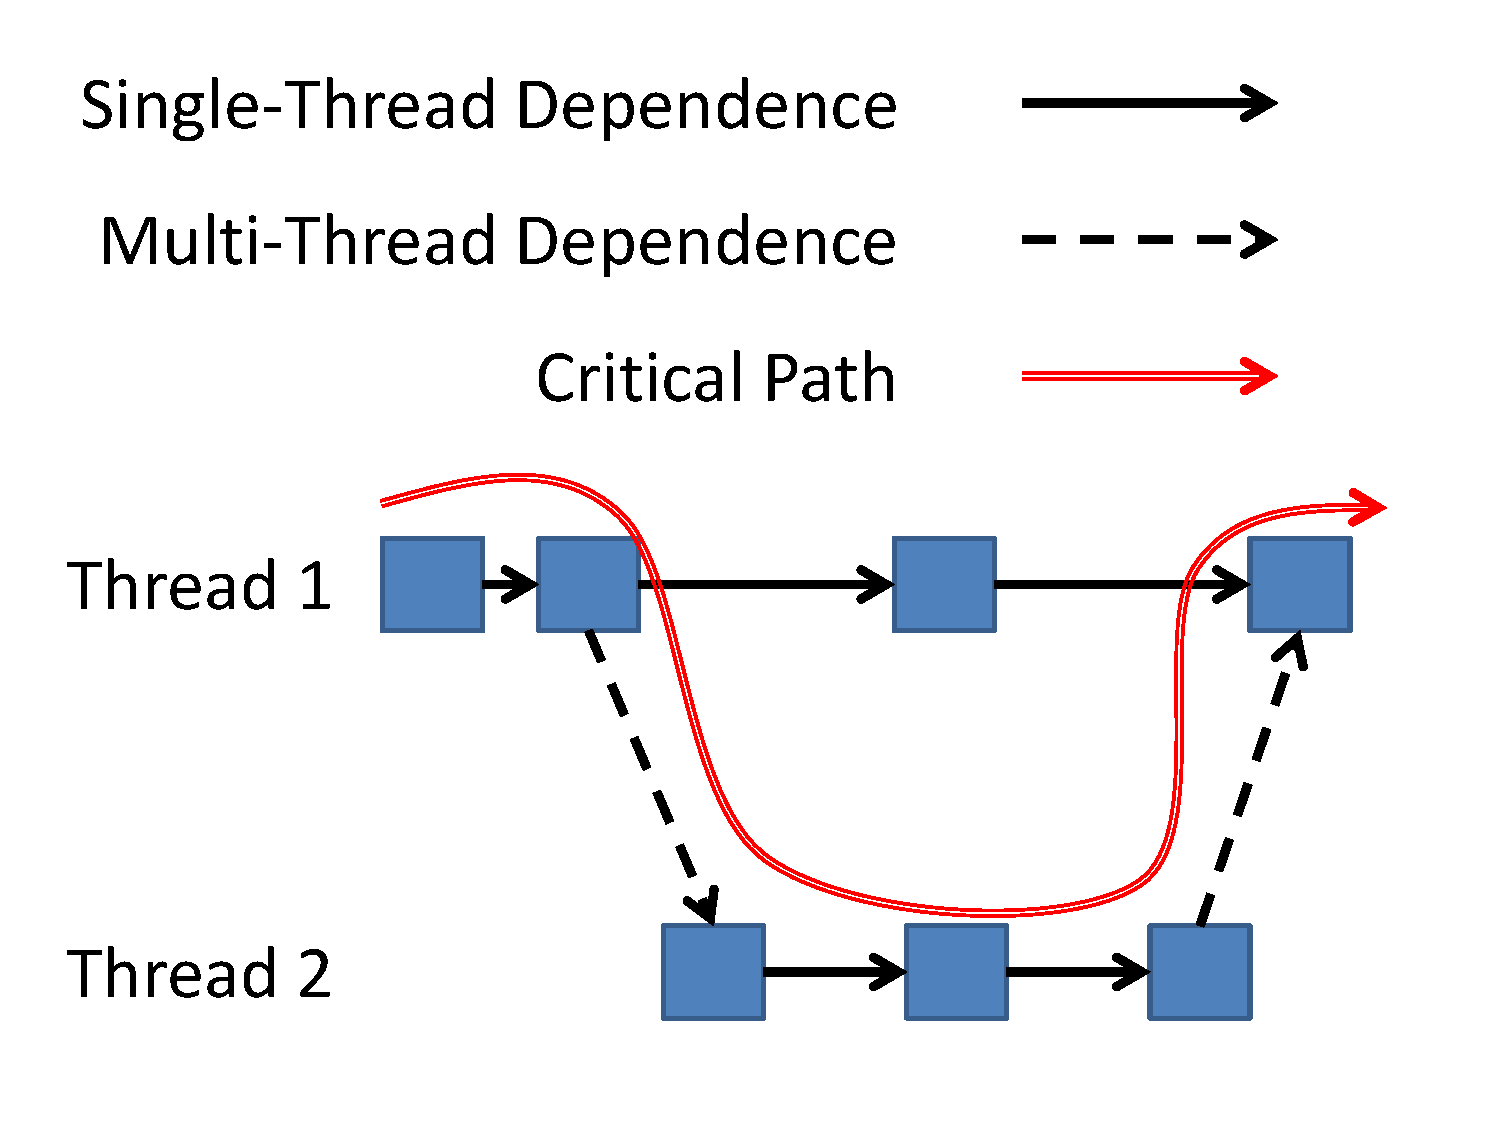
\includegraphics[width=.7\textwidth]{PMC/LPO.pdf}
\caption{\textbf{Local Persist Order.} LPO removes cross-thread persist dependencies, reducing persist critical path (PSC critical path traced in red).  Enforcing cross-thread dependencies requires explicit persist barriers.}
\label{figure:LPO}
\end{figure}

LPO potentially improves performance by minimizing the critical path of persist dependencies, shown in Figure~\ref{figure:LPO}
Data sharing and the resulting cross-thread persist dependencies increase the critical path of persists.
Even with buffering and high performance NVRAM memory systems that allow persists to buffer while threads continue, such chains limit throughput buffers become full, or increase delays caused by syncs while the buffers flush in persist-dependence order.
Since threads persist independently (except where persist barriers are placed), adding more threads provides more persist throughput, similarly to Symmetric Multi Threading (SMT), which provides memory parallelism on existing systems.
However, the need to perform all persists in serial within a thread remains a concern.
The Byte Addressable File System (BPFS) addresses intra-thread persist dependencies by introducing additional persist barriers.

\subsection{Byte Addressable Persistent File System}
\label{sec:PMC:PersistenceModels:BPFS}

The Byte Addressable Persistent File System (BPFS) \cite{ConditNightingale09} is the de-facto standard for existing persistent memory consistency models, used additionally by \cite{CoburnCaulfield11, FangHsiao11, VenkataramanTolia11}.
Threads persist by writing to the persistent address space, enforcing persist order via \emph{epoch barriers} which divide persists into \emph{epochs}.
BPFS additionally provides a hardware design, enforcing persist order with only cache modifications (little additionally buffering or modifications to the memory system).
A table of epochs is kept in the cache of each CPU, with each cache line keeping track of its persist epoch number and process/thread ID.
The cache writes back in the background, making sure that each epoch persists completely before starting to flush the next epoch.

Data sharing and persist order is enforced strictly by stalling.
If at any point a thread overwrites a cache line from a previous persist epoch (even from the same thread), it stalls until the previous persist epoch completes persisting.
Further, if a thread reads a cache line from a persist epoch produced by a remote thread that has not yet persisted it also stalls until that epoch completes persisting (it does not stall if the reading thread is the same as the producing thread).
Persists within epochs write to the device in parallel, volatile execution proceeds ahead of persistent state, and cross-thread persist order is correctly enforced (at the cost of stalls).

\begin{figure}
\centering
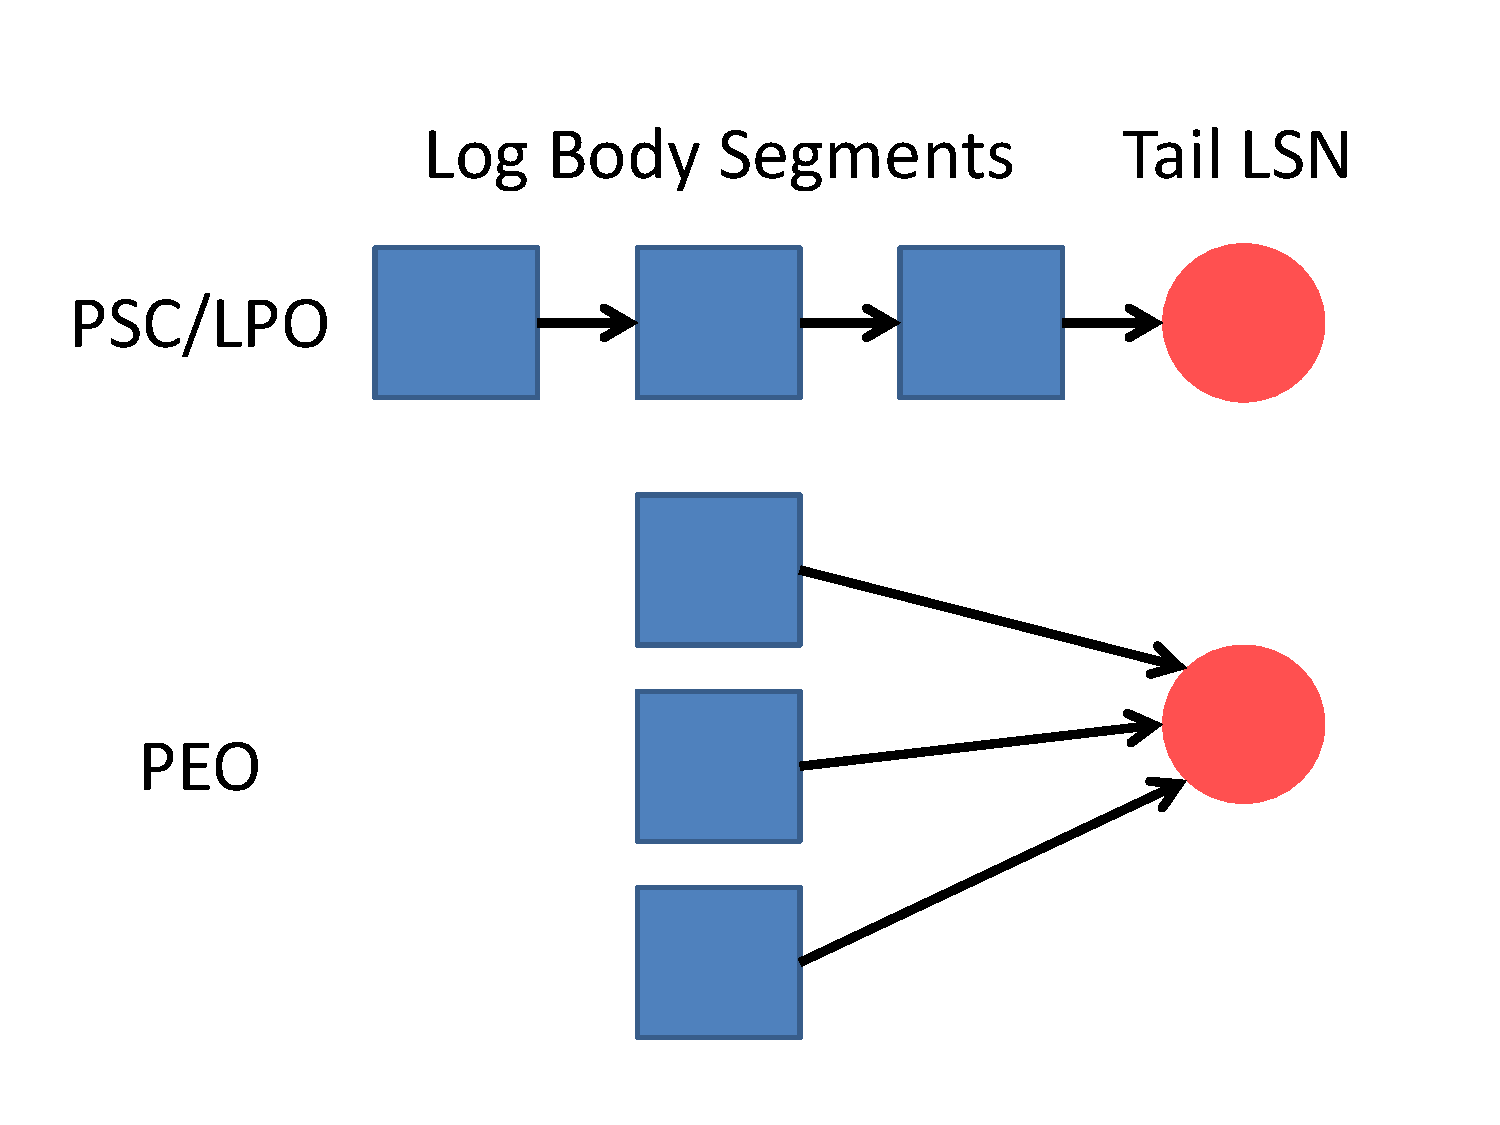
\includegraphics[width=.7\textwidth]{PMC/persist_wal.pdf}
\caption{\textbf{Partial Epoch Order.} PEO allows regions of NVRAM to persist in parallel while enforcing recovery correctness. \texttt{persist\_wal} persists entire log entry bodies in parallel using epochs.}
\label{fig:persist_wal_persist}
\end{figure}


Consider the ARIES log from Chapter~\ref{chap:OLTP_design}, demonstrated in \texttt{persist\_wal} (Figure~\ref{fig::Code}) with persist dependencies shown in Figure~\ref{fig:persist_wal_persist}.
Persisting a single entry requires first persisting the entry's body, followed by the tail LSN.
Most log entries are large (at least 100 bytes), containing information about the transaction, store, page, tuple, and action taken.
According to PSC and LPO all persists (8 byte segments) to the log entry body must occur in order -- an unnecessary constraint that increases persist critical path.
Instead, BPFS allows the entire log entry body to persist in parallel, and enforces that the body persists before the LSN using a persist barrier.

In consistency terms BPFS attempts to produce a total ordering of epochs that all threads observe (Total Epoch Order -- TEO -- would be a great name for this model).
This ordering resembles transactional memory -- producing a total order on memory transactions -- except BPFS does not provide conncurrenty control (transactions can not abort).
However, attempting to provide a total epoch order produces problems; multi-threaded BPFS execution may result in deadlock and restricts useful programming patterns.
I will demonstrate that the implementation as described is susceptible to deadlock.

{
\singlespacing
\newsavebox{\ThreadOne}
\begin{lrbox}{\ThreadOne}
  \begin{lstlisting}
Thread 1:

persist_bar
A = 1
B = 1
persist_bar
  \end{lstlisting}
\end{lrbox}

\newsavebox{\ThreadTwo}
\begin{lrbox}{\ThreadTwo}
  \begin{lstlisting}
Thread 2:

persist_bar
B = 2
A = 2
persist_bar
  \end{lstlisting}
\end{lrbox}

\begin{figure}[]
\centering
\subfigure{ \usebox{\ThreadOne} }
\hspace{1 in}
\subfigure{ \usebox{\ThreadTwo} }
\caption{\textbf{BPFS deadlock.} BPFS attempts to produce a total order on epochs.  Races within epochs create a cyclic order-dependence, resulting in deadlock.}
\label{fig:BPFS_deadlock}
\end{figure}
}

Consider Figure~\ref{fig:BPFS_deadlock}.
Each thread runs a single epoch with two persists to shared memory.
The second thread executes these persists in opposite order of the first.
If thread 1 writes to A at the same time thread 2 writes to B a deadlock occurs.
Thread 1 attempts to write to B, fetching the cache line for B, realizing that thread 2 has not yet persisted, so thread 1's epoch must be ordered after thread 2's epoch.
Similarly, thread 2 attempts to write to A, ordering its epoch after thread 1's; a cycle has occurred, preventing forward progress.

This problem may occur even without data races or when persists have a total order.
Imagine that A and B on each thread are different variables, each protected by locks, but that thread 1's A (B) is on the same \emph{cache line} as thread 2's A (B).
Such \emph{false sharing} may result in performance problems for existing volatile cache systems, but in the case of BPFS produces deadlock.
Furthermore, one might try to solve this problem by reordering thread 2's writes so that both thread 1 and thread 2 write in the same order, totally ordering the epochs (whoever accesses A first runs to completion while the other stalls).
However, relaxed consistency models allow the processor (or compiler) to reorder writes and persists within an epoch, arriving at the original problem.
In fact, it is not clear if instructions accessing only volatile data are permitted (or should be permitted) to reorder across epoch boundaries.
Finally, certain data structures may specifically intend to allow races within persist epochs.
The \GroupCommit implementation described above, for example, requires threads to work concurrently towards a persistent state.

BPFS attempts to produce a total order on all epoch barriers, producing deadlocks and preventing useful programming patterns.
I believe that the solution is to better define the interaction between persistence and the consistency model.
I next introduce a model strongly influenced by BPFS but that allows concurrent epochs to make forward progress at the cost of a slightly less intuitive interface.

\subsection{Partial Epoch Order}
\label{sec:PMC:PersistenceModels:PEO}

The third and final model relaxes persist order within a thread similarly to BPFS, but produces only a partial order of epochs between threads.
Partial Epoch Order (PEO) considers the epochs of two threads that communicate through memory to be \emph{concurrent}, and thus not ordered.
However, earlier and later epochs from those threads \emph{do} carry the dependence, allowing ordering of persists between threads while avoiding deadlock and allowing inter-thread persist concurrency.

{
\singlespacing
\newsavebox{\PEOThreadOne}
\begin{lrbox}{\PEOThreadOne}
  \begin{lstlisting}
Thread 1:

persist_bar (i)
persist A

persist_bar (ii)
persist X
write C

persist_bar (iii)
persist D
  \end{lstlisting}
\end{lrbox}

\newsavebox{\PEOThreadTwo}
\begin{lrbox}{\PEOThreadTwo}
  \begin{lstlisting}
Thread 1:

persist_bar (i)
persist B

persist_bar (ii)
read C
persist Y

persist_bar (iii)
persist E
  \end{lstlisting}
\end{lrbox}

\begin{figure}[]
\centering
\subfigure{ \usebox{\PEOThreadOne} }
\hspace{1 in}
\subfigure{ \usebox{\PEOThreadTwo} }
\caption{\textbf{Partial Epoch Order (PEO).} PEO considers epochs in different threads containing a memory dependence to be concurrent.  This memory dependence does not enforce a persist order between the threads' epochs, but enforces this order on earlier and later epochs.  E must persist after A.}
\label{fig:PEO}
\end{figure}
}

Figure~\ref{fig:PEO} provides an example.
Two threads persist data and communicate, each with three epochs.
Communication occurs in epoch (ii) of each thread -- thread 1 writes to (volatile) address C, which thread 2 reads.
According to PEO, epochs (ii) of each thread are concurrent and do not enforce a persist order.
Thus, thread 1's persist to X may not necessarily occur before thread 2's persist to Y.
However, epochs of thread 1 prior to (ii) must necessarily persist before epochs of thread 2 after (ii).
Thread 2's persist to A must persist before thread 2's persist to E.
The converse is not true -- thread 2's persist to B need not persist before thread 1's persist to D.
This model produces a single partial ordering of persist epochs that all threads observe.

It is unclear to me if volatile and non-memory instructions should be allowed to reorder with persist epoch barriers.
This will depend on the actual implementation, and if the hardware is able to easily distinguish persists from nonvolatile writes.
For example, thread 2's read to C in the previous example should be allowed to occur before the persist to B so long as the correct persist order is enforced.

PEO provides effective single-thread persist parallelism while providing a relatively intuitive model for cross-thread persist-order dependencies.
While not as intuitive as BPFS (total epoch order), PEO prevents deadlock and allows concurrent access to shared persistent memory spaces without enforcing a persist order when this is the desired behavior.

\section{Conclusion}
\label{sec:PMC:Conclusion}

This chapter motivated the need for more precise persistent consistency models to allow greater persist performance and enforce correctness while providing an easy to program interface.
I proposed three new persistent consistency models and relate them to existing work.
While this chapter has focused on persistence semantics and the programming interface, the next chapter demonstrates common persistent data structures, focusing on potential performance concerns.
